\documentclass[11pt,a4paper,ngerman]{report}
\usepackage{babel}
\usepackage{float}
\usepackage[utf8]{inputenc}
\usepackage[T1]{fontenc}
\usepackage{amsmath}
\usepackage{amssymb}
\usepackage{graphicx}
\usepackage{csquotes}
\usepackage[backend=bibtex,natbib=true,style=alphabetic]{biblatex}
\addbibresource{Quellen.bib}

\date{\today}
\title{Belegarbeit zur Quellenkodierungsmethode \textbf{"Run-Length Encoding"} im Modul "statistische Nachrichtentheorie"}

\author{Monique Golnik (563075)}






\begin{document}

	\maketitle
	\tableofcontents


	
	\chapter{Einleitung}
	
	1. Einleitungssatz
	2. Themavorstellung

	3. Ziel der Belegarbeit
	4. Aufbau der Hausarbeit


	\chapter{Quellenkodierung und Datenkompression}
	
		Bei der Quellkodierung ist es das Ziel, dass die Symbolentropie erhöht und so die Redundanz reduziert wird. Sie ist eine eineindeutige Darstellung der Quelleninformation in einer realisierbaren und möglichst redundanzfreien beziehungsweise -armen Form.
		
		Die Aufgabe der Quellenkodierung ist die Kodierung eines Datensatzes, der von einer Informationsquelle abgegeben wurde, in einen Binärcode mit möglichst kleiner Stellenzahl. \cite[Seite 47 ff.]{Lange2021}
	     
	    \enquote{Bei der Datenkompression werden Dateien in eine alternative Darstellung überführt, die effizienter ist als die ursprüngliche. Ziel dieser Codierung ist es, sowohl den benötigten Speicherplatz als auch die Übertragungszeit zu verringern.} \cite{IONOS} 
	
		Durch zwei unterschiedliche Ansätze, lässt sich so ein Codiergewinn erreichen:
	
		\begin{itemize}
		\item \textbf{Redundanz-Kompression}: 
		Auf der Grundlage einer Redundanzreduktion lassen sich Daten nach der Kompression verlustfrei wieder dekomprimieren - eine solche Kompression ist nur möglich, wenn ein Datensatz sich wiederholende Zeichen beinhaltet.
		
		\item \textbf{Irrelevanz-Kompression}:
		Bei diesem Ansatz werden irrelevante Informationen entfernt, um einen Datensatz zu komprimieren. Jedoch lässt sich dadurch der Datensatz nicht Bit-genau wiederhergestellten und ist somit verlustbehaftet
		\end{itemize}
	
	
		Im Folgenden wird der Blick auf die verlustfreie Kompressionsmethode \textbf{Run-Length Encoding} gerichtet und näher erläutert.
	
	
	\chapter{Run-Length Encoding}	
  		\section{Redundanz-Kompression durch \\ Run-Length Encoding}
  		  Die Lauflängencodierung \footnote{(Run-Length Encoding (RLE), Run-Length Coding (RLC), Lauflängencodierung = Synonyme} beschreibt eine verlustfreie Kompression, die sinnvoll angewandt werden kann, wenn der Datensatz Sequenzen mit sich mehrfach wiederholenden Zeichen enthält.
  		  
  		  
  		  Die RLE ist den sogenannten \textbf{Phrasencodern} zugeordnet, wie in Abbildung \ref{MMK} dargestellt.
  		  
  		  \begin{figure} [H]
  		  	\begin{center}
  		  		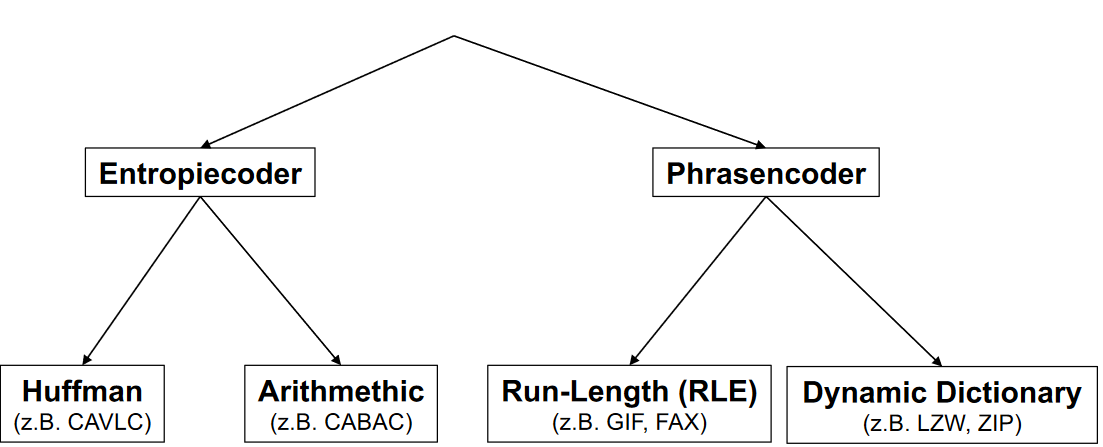
\includegraphics[width=0.75\textwidth]{MMK_RLE.png}
  		  		\caption{Klassifikation von verlustlosen Kompressionsmethoden}
  		  		\cite{MMK}
  		  		\label{MMK}
  		  	\end{center}
  		  \end{figure}
  		  
  		  
  		  Bei dieser Art der Codierung wird eine Folge von gleichen Zeichen, Buchstaben oder Zahlen durch ein Symbol und die Angabe über die Häufigkeit der gleichen Symbole substituiert. Die Abfolge von identischen Zeichen und der Länge der jeweiligen Sequenz, die in einem sogenannten Run Counter gespeichert wird, wird als \textbf{Run} bezeichnet. Diese Form der Kompression eignet sich sehr gut um Redundanzen in Grafiken und Bilddateien mit wenigen Farben zu beseitigen.

  		 %Formel richtig formatiert einfügen!
  	   	  %Aufeinanderfolgende Vorkommen eines Datensatze $d = Run$ (Lauf) \\
  	   	  
  	   	  %Anzahl der Wiederholungen $n$ von $d = RunLength$ (Lauflänge) \\
  	  
  	  
  		  Ist die zu komprimierende Grafik sehr detailreich, besitzt also sehr viele Farben oder Kontraste, ist die Lauflängencodierung nicht mehr geeignet,  da so nur sehr selten gleiche Zeichen in einer Sequenz aufeinander folgen.\cite{ITWissen.info} Auch für Texte eignet sich diese Methode eher nicht, da hier zwar Farben eine untergeordnete Rolle spielen, jedoch die aufeinander folgenden Buchstaben sehr selten gleich sind und so einzelne Zeichen nicht effizient zusammengefasst werden können.\cite[Seite 61]{Lange2021}
  		  
  		  Bei der Kompression werden identische Zeichen so lange eingelesen, bis sich einer ändert - Zeichen und Anzahl die gleich sind werden festgehalten. Bei der Dekompression wird der festgehaltene Wert ausgelesen und die dem entsprechende Anzahl an Bits ausgegeben.\cite{ITWissen.info}
  		  
  		  Sendet die Quellen neben Buchstaben auch Ziffern, so muss das Verfahren um Sonderzeichen erweitert werden, so dass die resultierende Angabe weiterhin eindeutig als Lauflänge gekennzeichnet ist. \cite[Seite 62]{Lange2021} Ein Beispiel zur Verdeutlichung findet sich in Abbildung \ref{Lange}.
  		  
  		   \begin{figure} [H]
  		  	\begin{center}
  		  		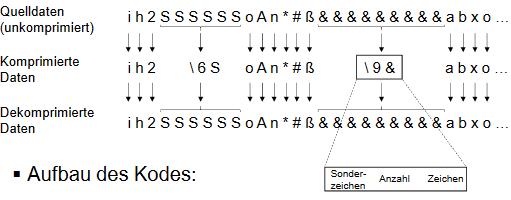
\includegraphics[width=0.75\textwidth]{alpha_ziffer.png}
  		  		\caption{Beispiel Verfahrenserweiterung}
  		  		\cite[Seite 62]{Lange2021}
  		  		\label{Lange}
  		  	\end{center}
  		  \end{figure}
  		  
  		  Der Kompressionsgrad des Run-Length Encodings hängt stark von der Charakteristik der Quelldaten ab. \cite[Seite 62]{Lange2021}
  		  
  		 % Sonderfall binärcode hinzufügen
  		 
  		 
	
		\section{Vor- und Nachteile gegenüber anderen Verfahren}
		%Vorteile
		Das RLE-Verfahren zeichnet sich durch seine Geschwindigkeit und Einfachheit aus.
		reversibel
		verlustfrei gegenüber bsp huffman
		
		%Nachteile
		keine optimale Redundanzreduktion
		
		
		
		
		
		\section{Einsatz}
		Die Lauflängencodierung findet Anwendung bei verschiedenen Grafikdateiformaten, wie beispielsweise dem TIFF \footnote{TIFF = Tagged Image File Format}, dem TGA- und dem Bitmap-Dateiformat.
		
		In der Computergrafik wird das Lauflängencodierungs-Verfahren bei speicherintensiven Rastergrafiken angewendet und ist besonders effizient, wenn es sich um Grafiken mit wenigen aber großflächigen Farben handelt. Das Verfahren kann dabei sogar noch optimiert werden, in dem eine Wegoptimierung durch die Wahl des effektivsten Laufweges anhand eines Algorithmus vorgenommen wird.  Dieser Laufweg könnte beispielsweise zeilen-sequenziell, im Zick-Zack siehe Abbildung \ref{zickzack} oder mäanderförmig \footnote{Mäander = Bezeichnung einer Flussschlinge in einer Abfolge weiterer Flussschlingen } siehe Abbildung \ref{mäander} sein.
		
		
		 \begin{figure} [H]
			\begin{center}
				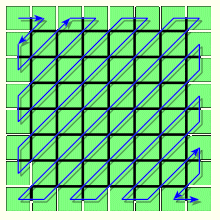
\includegraphics[width=0.25\textwidth]{zickzack.png}
				\caption{Wegoptimierung: Zick-Zack}
				\cite{rostfrank}
				\label{zickzack}
			\end{center}
		\end{figure}
		
		 \begin{figure} [H]
			\begin{center}
				\includegraphics[width=0.25\textwidth]{Mäander.png}
				\caption{Wegoptimierung: Mäanderförmig}
				\cite{kocerheiztech}
				\label{mäander}
			\end{center}
		\end{figure}
		
		
		\section{Anwendungsbeispiele}
		gymnasium westerstede hat beispiele
		
		
		  \begin{figure} [H]
			\begin{center}
				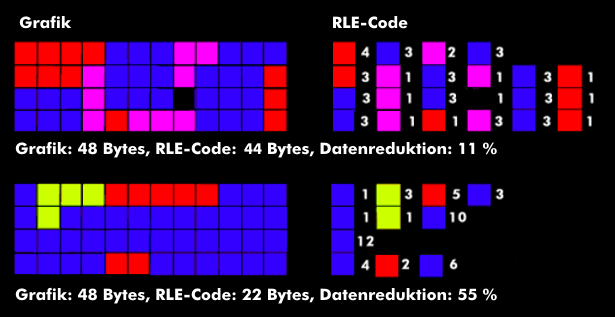
\includegraphics[width=0.75\textwidth]{g_h_Effizienz.png}
				\caption{Beispiel mit geringer und höherer Effizienz}
				\cite{ITWissen.info}
				\label{Effizienz}
			\end{center}
		\end{figure}
		
		
	
	\chapter{Fazit}
	
	\chapter{Eigenständigkeitserklärung}
	
	Hiermit versichere ich, dass ich die vorliegende Belegarbeit selbstständig und nur unter
	Verwendung der angegebenen Quellen und Hilfsmittel verfasst habe. Die Arbeit wurde bisher
	in gleicher oder ähnlicher Form keiner anderen Prüfungsbehörde vorgelegt.
	
	\vskip 1cm
	
	Berlin, den \date{\today}
	
	\vskip 1.5cm
	
	Monique Golnik
	
		
	\listoffigures
	
	
	\printbibliography[heading=bibintoc, keyword={online}, title={Onlinequellen}]\clearpage
	\printbibliography[heading=bibintoc, keyword={image}, title={Bildquellen}]\clearpage
	
\end{document}
